\section{Problem 2}
\textit{Consider the random process $x[n]$ created as $x[n] = 4w[n] - 2w[n-3]$ Where
w[n] is unit variance white Gaussian noise.}

\subsection{1.}
\textit{Compute an analytic expression for the autocorrelation $r_{xx}[l]$}\\
The definition of the autocorrelation, how a signal correlates to itself, takes the 
form of 
\[r_{xx}[l] = \textbf{E}\{x[n]x[n-l]\} \]
Inserting the given expression of $x[n]$ into the autocorrelation definition yields a rather length expression:
\[
r_{xx}[l] =
\textbf{E}\{(4w[n] - 2w[n-3])\cdot(4w[n-l] - 2w[n-l-3])\}
\]
expanding
\[
r_{xx}[l] = 
\textbf{E}\{
16w[n]w[n-l]
- 8w[n]w[n-l-3]
- 8w[n-3]w[n-l]
+ 4w[n-3]w[n-l-3]
\}
\]
Since $w[n]$ is described as being unit variance white gaussian noise, we 
also make the assumption that the noise is zero-mean.
Unit variance meaning that the variance $\sigma^2 = 1$. Because of this, we
can write the definition of the autocorrelation of white noise
\[
\textbf{E}\{x[n]x[n-l]\} = \sigma^2\delta[l]
\]
we can then apply this rule to every expectation and move the coefficients to each term, and making
makes the difference between each sample index equal to zero. essentially we want the argument of the 
delta function to become zero and it follows the rule:
\[
\delta[l] = \begin{cases}
    \sigma^2, & \text{if } l = 0\\
    0, & \text{if } l \neq 0
\end{cases}
\]
\[\text{first term:} \]
\[16\textbf{E}\{w[n]w[n-l]\} = \delta[l] \Rightarrow 16\delta[l]\]
\[\text{second term:}\]
\[ n = n - l - 3 \Rightarrow l = -3 \Rightarrow \delta[l+3]\]
\[-8\textbf{E}\{w[n]w[n-l-3]\} = \delta[l]\Rightarrow -8\delta[l+3]\]
\[\text{third term:}\]
\[ n - 3 = n - l \Rightarrow l = 3\]
\[-8\textbf{E}\{w[n-3]w[n-l]\} = \delta[l] \Rightarrow -8\delta[l-3]\]
\[\text{fourth term:}\]
\[ n - 3 = n - l - 3 \Rightarrow l = 0 \]
\[4\textbf{E}\{w[n-3]w[n-l-3]\} = 4\delta[l]\]
Combining the terms:
\[r_{xx}[l] = 20\delta[l]-8\delta[l+3]-8\delta[l-3]\]
This leads to the autocorrelation:
\[
r_{xx}[l] = \begin{cases}
    20, & l = 0\\
    -8, & l = \pm3\\
    0, & \text{otherwise} 
\end{cases}
\]


\subsection{2.}
\textit{Plot the power spectral density of the random process. What can be learned from the plot?}\\
The \textit{PSD} of a stationary random signal, is the fourier transform of the 
autocorrelation, which shows the distribution of power as a function of frequency.
It can be calculated using:
\[S_{xx}(e^{j\omega}) = \sum_{l=-\infty}^{\infty}r_{xx}[l]e^{-jl\omega}\]
If this is applied to $r_{xx}$ from before, we can see that we only have conditions
for $l$ in 3 cases, all other cases the summation term becomes zero. Thus it can
be expressed as:
\[S_{xx}(e^{j\omega}) = r_{xx}[-3]e^{-j(-3)\omega} + r_{xx}[-0]e^{-j0\omega} + r_{xx}[3]e^{-j3\omega}\]
\[\Downarrow\]
\[= 20e^{j0\omega} - 8e^{-j(-3)\omega} - 8e^{-j3\omega}\]
\[\Downarrow\]
\[= 20 - 8e^{j3\omega} - 8e^{-j3\omega}\]
this can be rewritten using euler identities relating euler complex functions to sinusoids.
\[= 20 - 8(e^{j3\omega} + e^{-j3\omega})\]
\[\Downarrow\]
\[= 20 - 8(\cos(3\omega) + j\sin(3\omega) + \cos(3\omega) - j\sin(3\omega)) \]
\[\Downarrow\]
\[= 20 - 8(2cos(3\omega))\]
\[\Downarrow\] 
\[= 20 - 16\cos(3\omega)\]
which can be plotted:
\begin{figure}[!htb]
    \centering
    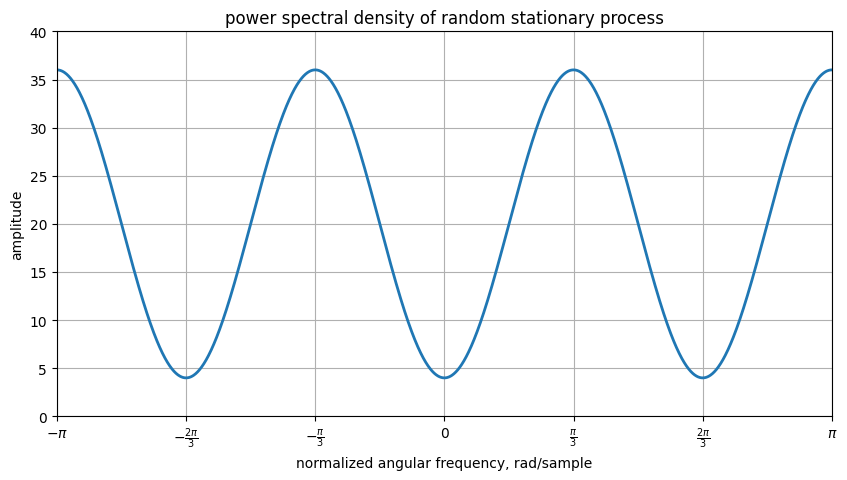
\includegraphics[width=0.6\textwidth]{opg_2_PSD.png}
    \caption{power spectral density depicts a sinusoid, which means it is periodic}
\end{figure}

\subsection{3.}
\textit{Assume $x[n]$ is filtered through a FIR filter with $H(z) = 5+z^{-1}$}\\
\textit{Compute the analytical expressions for $r_{yx}[l]$ and $r_{yy}[l]$}

% Firstly, were given the filter in the z-domain, where the filter essentially tells us \textit{"take the current samples
% and multiply by 5 and add it to the previous input sample"} this can be constructed as 
% \[y[n] = 5x[n] + x[n-1]\]
% It is then possible to put our definition of $x[n]$ into this filter and for the second term shift all n-samples by 1
% \[y[n] = 5 \{4w[n]-2w[n-3]\} + \{4w[n-1]-2w[n-4]\} \Rightarrow 20w[n] + 4w[n-1] - 10w[n-3]-2w[n-4]\] 
% To find $r_{yx}$, which is the cross-correlation, between y and x, meaning how much
% two signals are alike when shifted relative to eachother, has the definition:
% \[y_{yx}[l] = \textbf{E}\{y[n]x[n-l]\}\]
% It is then possible to substitute the filter function into the\\ 

% ALTERNATIVT\\
Firstly, were given the filter in the z-domain, where the filter essentially tells us \textit{"take the current samples
and multiply by 5 and add it to the previous input sample"} which can be inverse z-transformed to yield:
\[h[l] = 5\delta[l] + \delta[l-1]\]
It is then possible to use the formula described in (13.100), and because we found $r_{xx}$ earlier
\[r_{yx}[l] = h[l] * r_{xx}[l]\]
Using the impulse-convolution rule and substituting $h[l]$ and $r_{xx}$ into the convolution using $\delta[l-a] * \delta[l-b] = \delta[l-(a+b)]$, yielding six impulse terms.
\[r_{yx}[l] = (5\delta[l]+\delta[l-1]) * (20\delta[l]-8\delta[l+3]-8\delta[l-3])\]
\[\Downarrow\]
\[5\delta[l] * 20\delta[l] = 100\delta[l]\]
\[5\delta[l] * (-8\delta[l-3]) = -40\delta[l-3]\]
\[5\delta[l] * (-8\delta[l+3]) = -40\delta[l+3]\]
\[\delta[l-1]* 20\delta[l] = 20\delta[l-1]\]
\[\delta[l-1]* (-8\delta[l-3]) = -8\delta[l-4]\]
\[\delta[l-1]* (-8\delta[l+3]) = \delta[l-1] * (-8\delta[l-(1+(-3))]) = -8\delta[l+2]\]
\[\text{summing all terms:}\]
\[r_{yx}[l] = 100\delta[l] + 20\delta[l-1] - 40\delta[l-3] - 40\delta[l+3] -8\delta[l-4] -8\delta[l+2]\]

To find $r_yy$, equation 13.111 from the book can be used
\[R_{yy} = H(Z)H(\frac{1}{Z})R_{xx}(Z)\]
This requires us to use $R_{xx}(Z)$, meaning a z-transform of $r_{xx}(l)$ is required.
The functions then becomes:
\[H(Z) = 5+Z^{-1}\]
\[H(\frac{1}{Z}) = \frac{1}{5+Z^{-1}} \Rightarrow  5 + \frac{1}{\frac{1}{Z}} = 5+Z\]
For Z-transformation:
\[Z(\delta(l-k)) = z^{-k}\]
\[r_{xx}[l] = 20\delta[l]-8\delta[l+3]-8\delta[l-3]\]
\[\Downarrow Z-trans\]
\[R_{xx}[Z] = 20 -8Z^{3}-8Z^{-3}\]
Combining all the expressions:
\[R_{yy} = (5+Z^{-1})(5+Z)(20 -8Z^{3}-8Z^{-3})\]
Solved using CAS tool
\[\Downarrow\]
\[R_{yy}[Z] = (- 40z^{4}) -208z^{3} -40z^{2} + 100z+ 520  + 100z^{-1} - 40z^{-2} - 208z^{-3}-40z^{-4}\]
Inverse Z-transform to get $r_{yy}[l]$
\[r_{yy}[l] = (- 40\delta(l+4)) -208\delta(l+3) -40\delta(l+2) + 100\delta(l) + 520  + 100\delta(l-1) - 40\delta(l-2) - 208\delta(l-3)-40\delta(l-4)\]

